
%(BEGIN_QUESTION)
% Copyright 2006, Tony R. Kuphaldt, released under the Creative Commons Attribution License (v 1.0)
% This means you may do almost anything with this work of mine, so long as you give me proper credit

Shown here is a diagram of a standard pressure gauge, based on the pressure-sensing action of a hollow, C-shaped metal tube called a {\it bourdon tube}:

$$\includegraphics[width=15.5cm]{i00173x01.eps}$$

Using arrows, trace the motions of all moving components in this mechanism as an increasing pressure is applied to the fitting at the bottom of the bourdon tube.

\vskip 10pt

Also, describe how the measurement span of this pressure gauge could be changed.  In other words, what would have to be moved, adjusted, or altered in this mechanism in order to change the proportionality of applied pressure to pointer movement?

\vskip 20pt \vbox{\hrule \hbox{\strut \vrule{} {\bf Suggestions for Socratic discussion} \vrule} \hrule}

\begin{itemize}
\item{} Questions such as this tend to be challenging for people with limited experience working on mechanical devices.  Identify some problem-solving strategies for a mechanically innocent student to apply to problems such as this.
\item{} What sort of device(s) would you suggest using to apply a precisely known pressure to a gauge for calibration purposes?
\item{} Suppose a pressure gauge is intended for service in a process measuring liquid pressure.  Is it okay to calibrate this gauge on a test bench using compressed {\it air} instead of the liquid it will be exposed to in the field?  Why or why not?
\end{itemize}

\underbar{file i00173}
%(END_QUESTION)





%(BEGIN_ANSWER)

The parts in this gauge mechanism would move as such:

$$\includegraphics[width=15.5cm]{i00173x02.eps}$$

Possible things to change to make this pressure-measuring mechanism more sensitive:

\begin{itemize}
\item{} Decrease the spring rate (``stiffness'') of the bourdon tube
\item{} Shorted the arm of the sector gear (the portion to the right of the pivot, joining with the link)
\item{} Increase the sector gear radius
\item{} Decrease the pinion gear radius
\end{itemize}

%(END_ANSWER)





%(BEGIN_NOTES)

As the tip of the bourdon tube moves up and to the right, it pulls on the link, moving the right-hand end of the sector up.  This turns the sector gear counter-clockwise on its pivot, which will turn the pinion gear clockwise.  This clockwise motion drives the pointer clockwise up the pressure scale (not shown).

I strongly recommend bringing a bourdon tube pressure gauge to class for inspection!  Even better than a gauge by itself is a gauge mounted on a deadweight tester, so students can see the bourdon tube mechanism in operation as you increase and decrease pressure.

\vskip 10pt

The Wika gauge company has a great video on YouTube showing the manufacture and testing of a bourdon tube pressure gauge, well worth showing to the class.

%INDEX% Measurement, pressure: bourdon tube

%(END_NOTES)


